\begin{figure}[ht]
\centering

\begin{subfigure}[t]{0.45\textwidth}
\centering
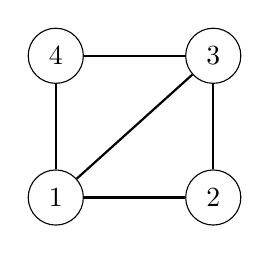
\begin{tikzpicture}[
  v/.style={circle, draw, minimum size=7mm},
  e/.style={thick}
]
\node[v] (1) at (0,0) {1};
\node[v] (2) at (2,0) {2};
\node[v] (3) at (2,1.8) {3};
\node[v] (4) at (0,1.8) {4};

% undirected edges
\draw[e] (1)--(2);
\draw[e] (2)--(3);
\draw[e] (3)--(4);
\draw[e] (4)--(1);
\draw[e] (1)--(3);
\end{tikzpicture}
\caption{Undirected graph on 4 nodes}
\label{fig:undirected4}
\end{subfigure}
\hfill
\begin{subfigure}[t]{0.45\textwidth}
\centering
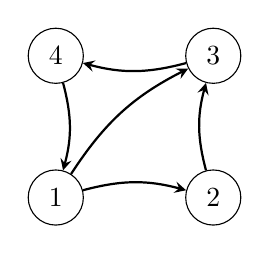
\begin{tikzpicture}[
  v/.style={circle, draw, minimum size=7mm},
  e/.style={thick, ->, >=stealth}
]
\node[v] (1) at (0,0) {1};
\node[v] (2) at (2,0) {2};
\node[v] (3) at (2,1.8) {3};
\node[v] (4) at (0,1.8) {4};

% directed edges
\draw[e] (1) to[bend left=15] (2);
\draw[e] (2) to[bend left=15] (3);
\draw[e] (3) to[bend left=15] (4);
\draw[e] (4) to[bend left=15] (1);
\draw[e] (1) to[bend left=15] (3);
\end{tikzpicture}
\caption{Directed graph on 4 nodes}
\label{fig:directed4}
\end{subfigure}

\caption{Examples of (a) undirected and (b) directed graphs on four nodes.}
\label{fig:two-graphs}
\end{figure}